\chapter{Risk Management: Options and Corporate Finance}

\section{Introduction}

Topics:
\begin{itemize}
    \item Describe the basics of using options in risk management
    \item Identify what drives the value of options (intrinsic and speculative values)
    \item Examine the different strategies to build funds, including options
\end{itemize}

\section{Equity and Debt as Options}

\begin{itemize}
    \item Options provide valuable insights into corporate finance concepts, particularly in understanding debt and equity.
    \item \textbf{Equity} can be conceptualised as a \textbf{long call option on a firm's assets} with a strike price equivalent to the value of debt:
      \begin{itemize}
        \item If the firm's value exceeds the debt, equity holders benefit from the residual value post-debt repayment.
        \item If not, equity holders lose their investment, similar to an option expiring worthless.
      \end{itemize}
      \begin{figure}[H]
        \centering
        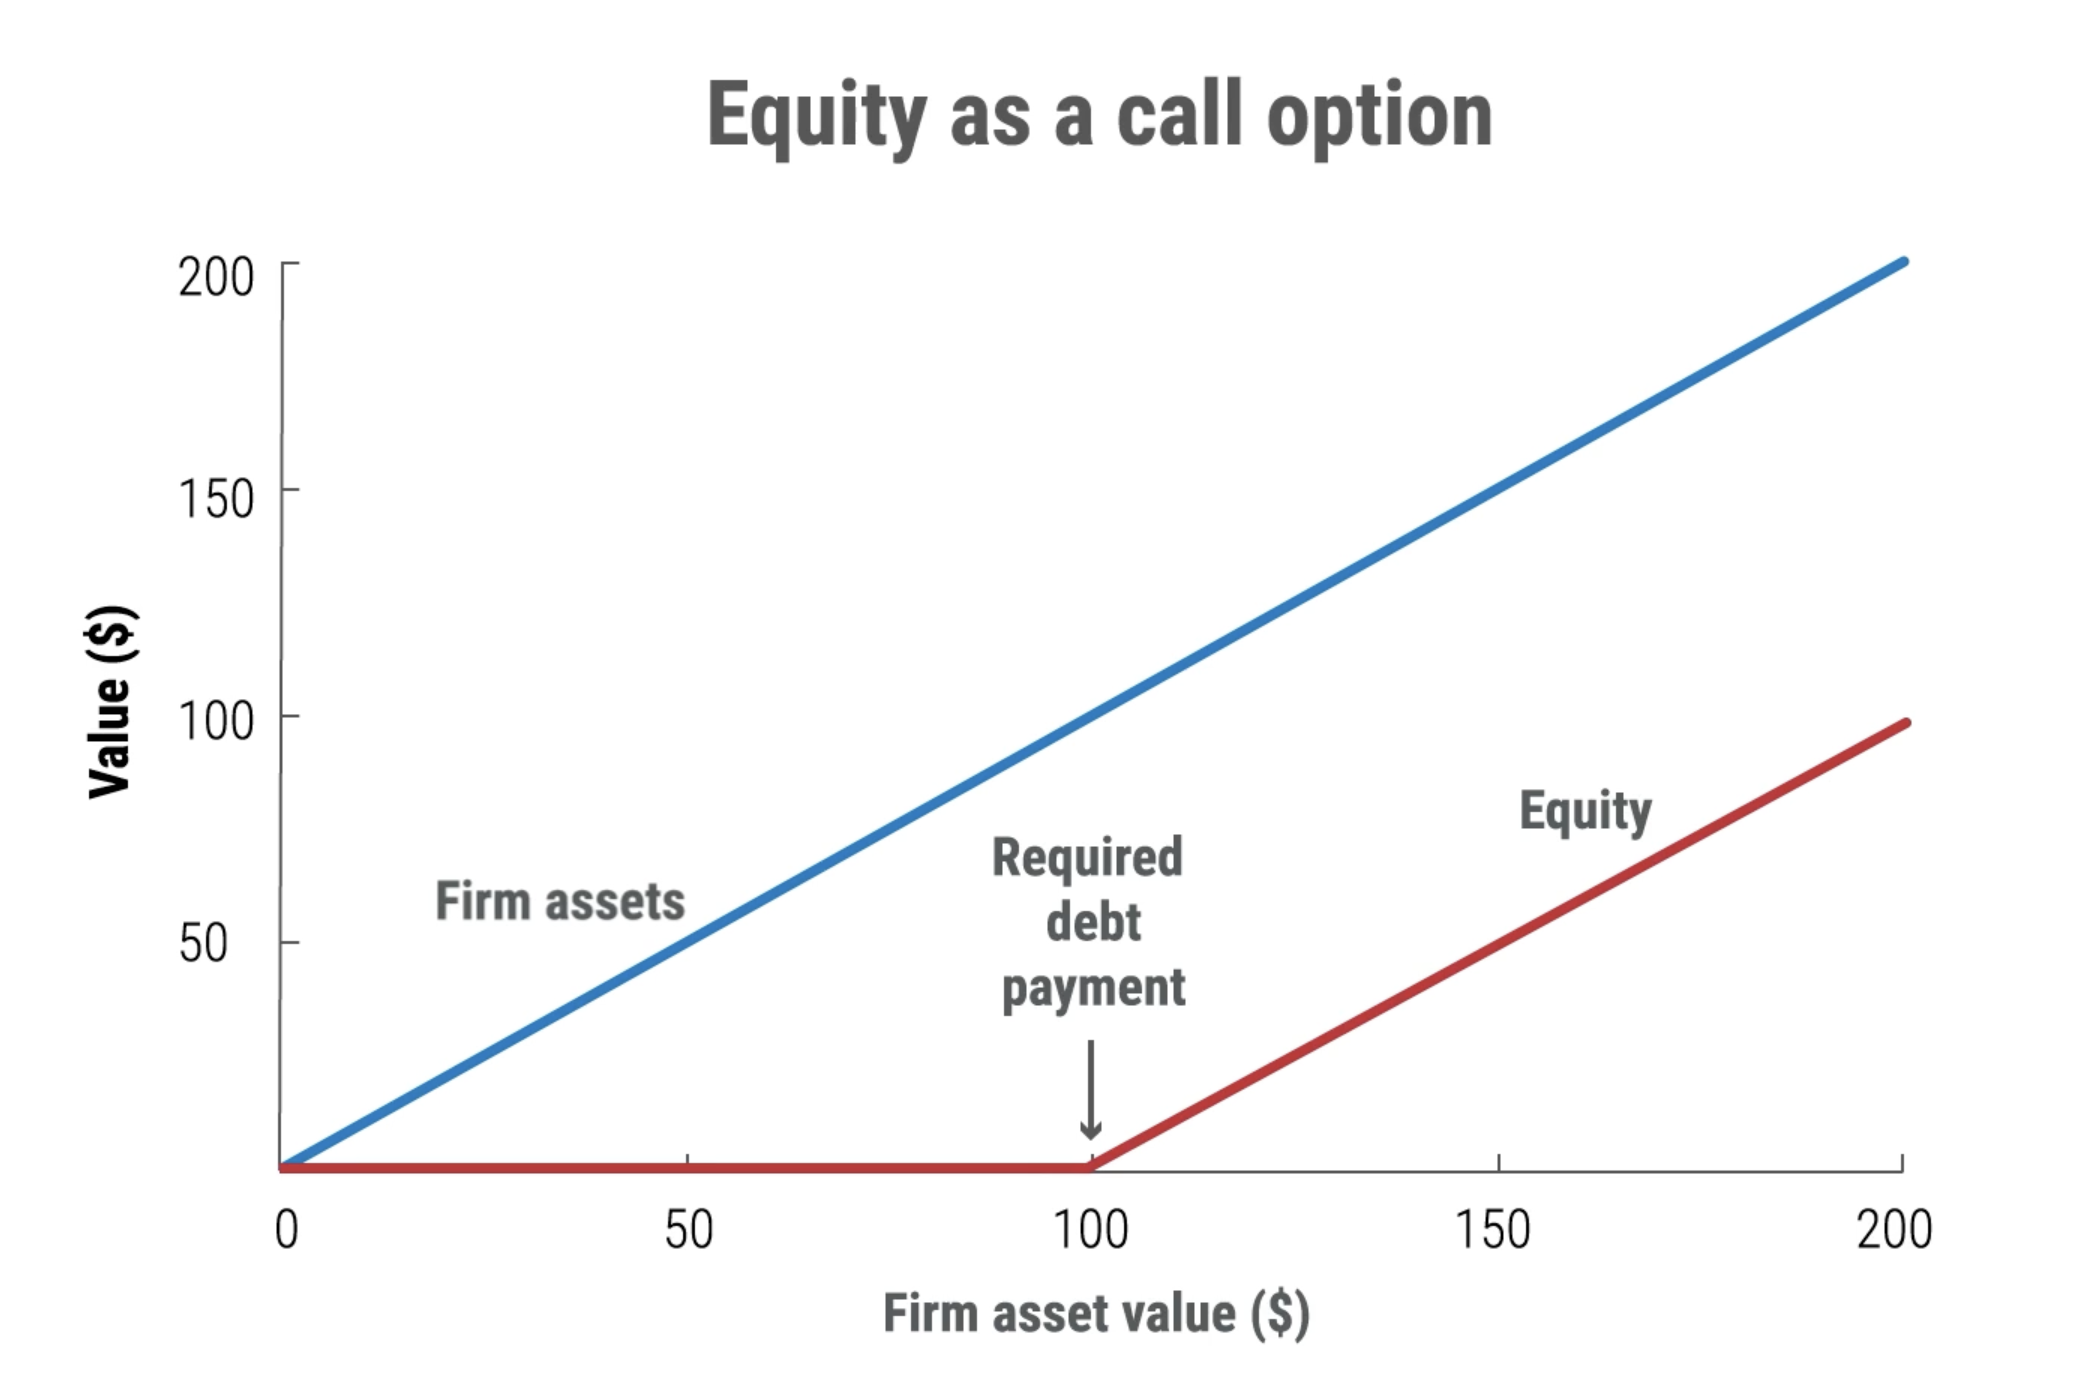
\includegraphics[width=0.5\textwidth]{img/10.2.1.png}
        \caption{Equity as a Call Option}
        \end{figure}
    \item Equity shares resemble call options in several ways:
      \begin{itemize}
        \item They offer limited risk, capping potential losses to the initial investment.
        \item They provide unlimited upside, allowing equity holders to benefit fully from increases in the firm's value.
        \item Unlike traditional options, equity does not expire, permitting long-term value appreciation.
      \end{itemize}
    \item \textbf{Debt} can also be analysed using options theory:
      \begin{itemize}
        \item It can be seen as a \textbf{short put option on the firm's assets with a strike price equal to debt}.
        \item If asset values fall below the debt level, the put option is exercised, leaving debt holders with the firm's remaining assets.
        \item If asset values exceed the debt, debt holders receive only the debt amount, similar to a call option's strike price being met.
      \end{itemize}
      \begin{figure}[H]
        \centering
        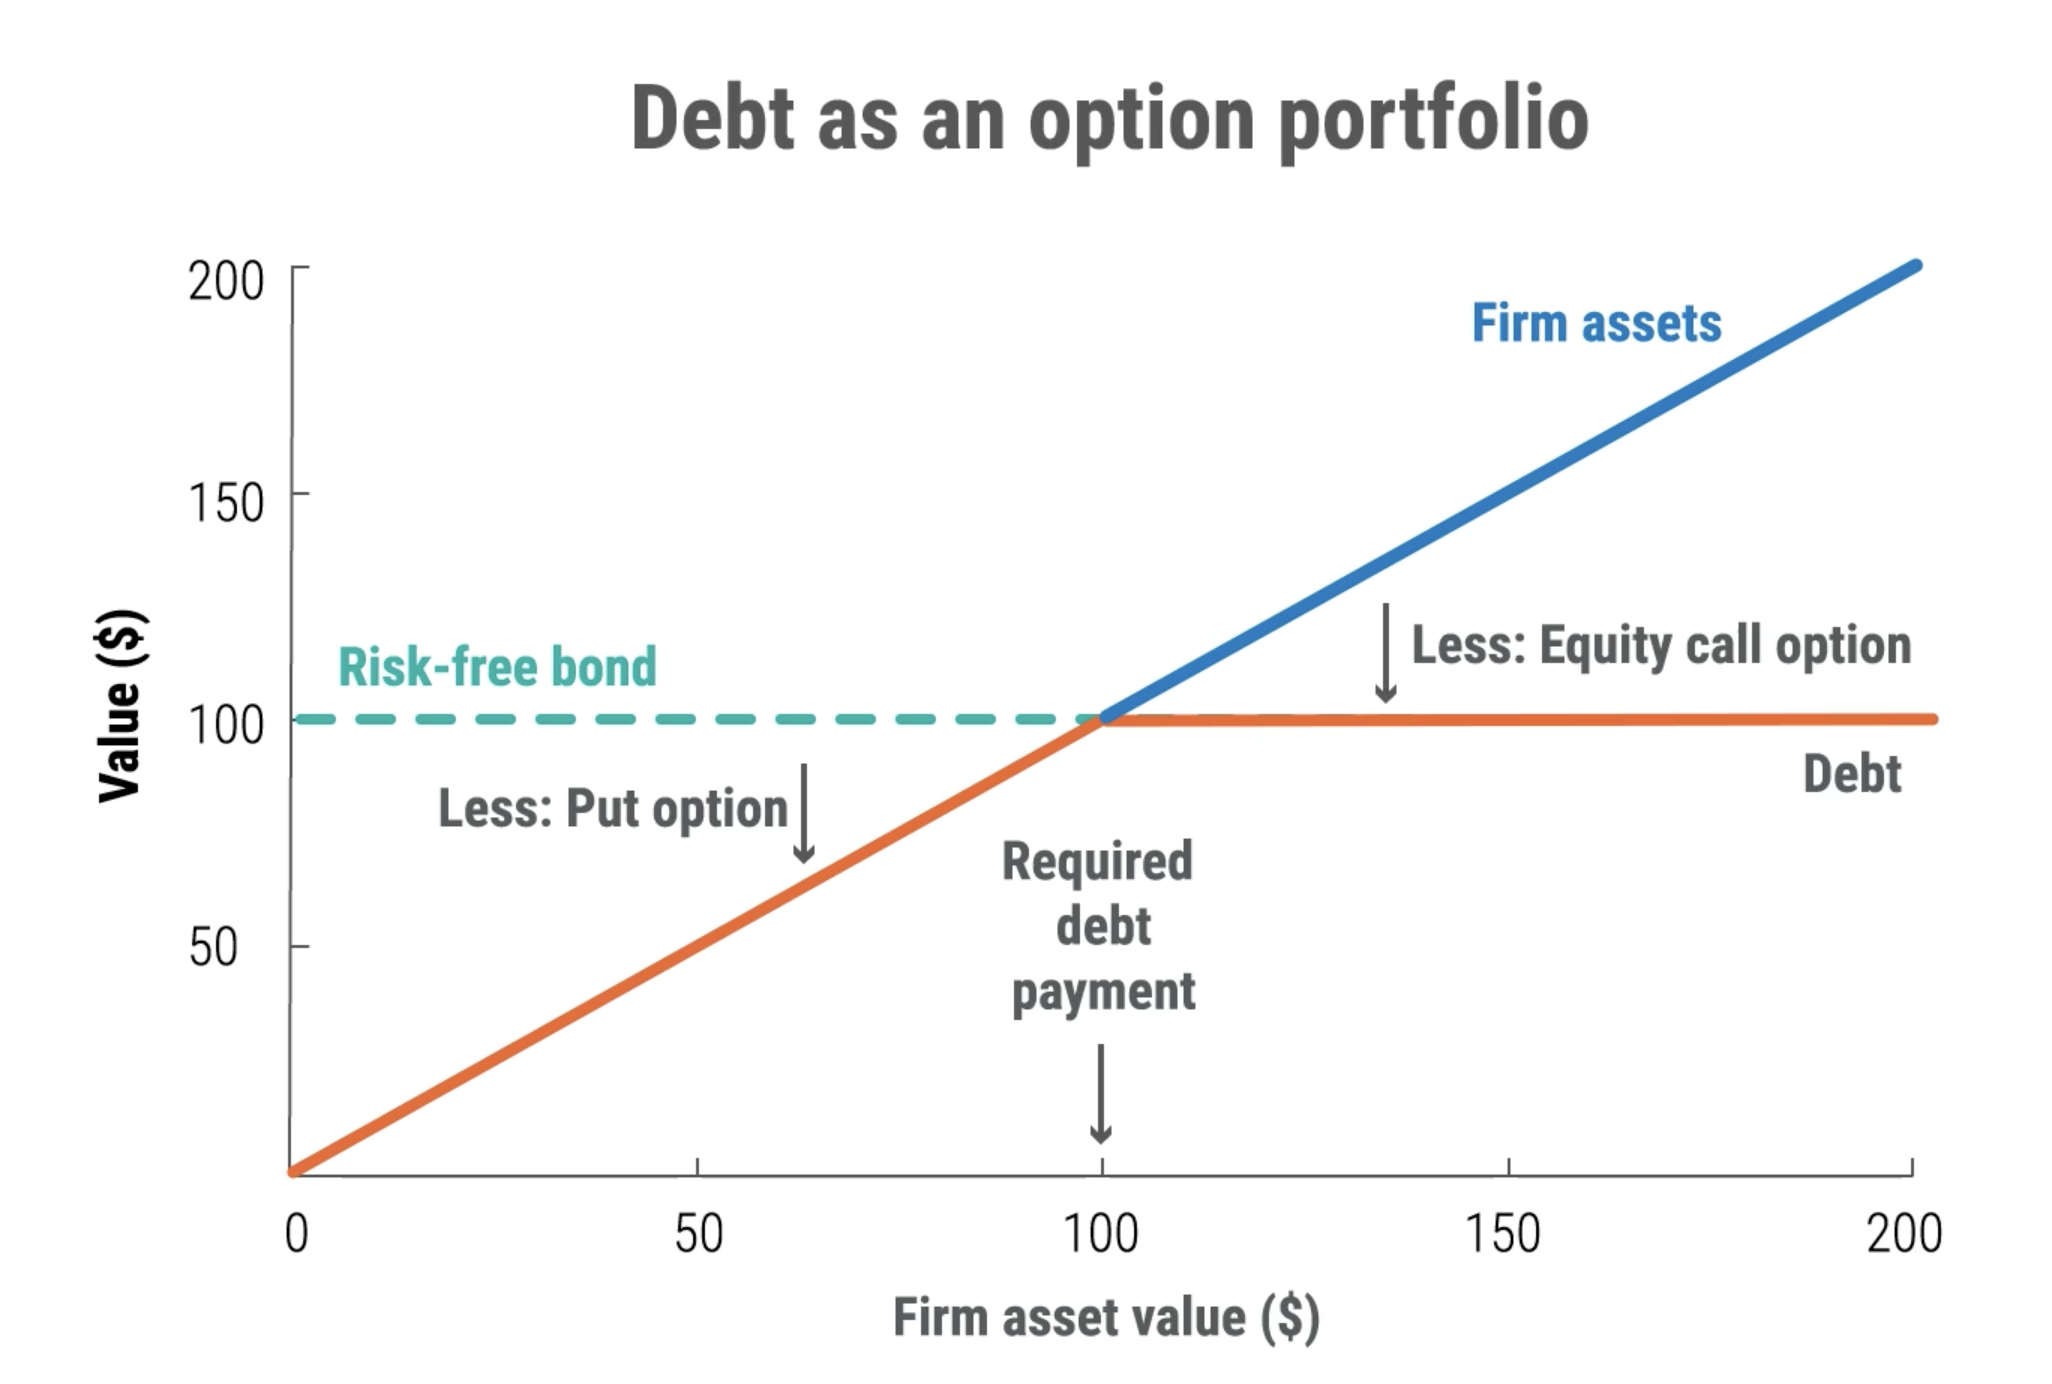
\includegraphics[width=0.5\textwidth]{img/10.2.2.png}
        \caption{Debt as a Put Option}
        \end{figure}
  \end{itemize}
  
\section{Agency Conflict}
\subsection*{Debt Equity Considered as Options}

% \begin{itemize}
%     \item Viewing debt equity as options provides a methodological framework for pricing securities.
%     \item Useful in situations where a company has traded options but no outstanding debt, assisting in pricing a debt issue.
%     \item The option characterisation of debt and equity securities offers a new perspective on agency conflicts between equity holders and debt holders.
%     \item These conflicts may lead to:
%     \begin{itemize}
%         \item Overinvestment or underinvestment issues.
%         \item Divergent attitudes towards risk due to equity's similarity to a call option:
%         \begin{itemize}
%             \item Equity holders benefit from risky investments, reflecting a preference for higher risk (akin to holding a long call option).
%             \item Conversely, this positions equity holders similarly to short put option holders, where increased risk is detrimental.
%         \end{itemize}
%     \end{itemize}
%     \item Such dynamics can lead to an over-investment problem:
%     \begin{itemize}
%         \item New investments that enhance asset values can decrease the value of the effective short put held by equity holders.
%         \item This reduction in put value means that some benefits of asset value increase are transferred to debt holders, diminishing equity holders' incentives to invest.
%     \end{itemize}
%     \item The shift in incentives can result in:
%     \begin{itemize}
%         \item A debt overhang, where the potential gains from new investments accrue more to debt holders than to equity holders.
%         \item An underinvestment problem, as equity holders perceive reduced benefits from investment.
%     \end{itemize}
% \end{itemize}


\begin{itemize}
    \item Thinking of debt and equity as options can help price securities, especially when a company has traded options but no debt outstanding. This is because options pricing models can be used to estimate the value of debt and equity, providing a more accurate picture of a company's capital structure.
    \item This perspective provides a new interpretation of agency conflicts between equity holders and debt holders. By recognizing that debt and equity have option-like characteristics, we can better understand the incentives and conflicts that arise between these two groups.
    \item Equity can be viewed as a call option, giving equity holders a potential upside from investments. This is because equity holders benefit from any increase in the firm's value, making their claim on the firm's assets more valuable.
    \item However, debt holders have a short put option position, which means they are hurt by increased risk. This is because debt holders are obligated to receive a fixed return, and any increase in risk reduces the value of their claim on the firm's assets.
    \item This can lead to:
        \begin{itemize}
            \item Overinvestment: Equity holders may take on excessive risk, as they benefit from potential gains and have limited liability. This can lead to a moral hazard problem, where equity holders take on too much risk at the expense of debt holders.
            \item Underinvestment: Debt holders may be hesitant to invest, as increased risk reduces the value of their put option. This can lead to a debt overhang problem, where debt holders are reluctant to provide financing for new projects.
        \end{itemize}
    \item When a firm makes new investments, the value of the debt (short put option) increases, as the assets backing the debt become more valuable. This means that debt holders benefit from the increased asset value, as their claim on the firm's assets becomes more secure.
    \item When debt holders benefit from increased asset value, equity holders may be less inclined to invest in new projects, as the benefits of those investments may accrue primarily to debt holders. This can lead to a debt overhang problem, where equity holders are hesitant to invest in projects that could increase the firm's value.y be less inclined to invest, as they may not capture the full benefits of their investments. This is known as the debt overhang problem or underinvestment problem, where equity holders may be hesitant to invest in projects that could increase the value of the firm, as the benefits may accrue to debt holders instead.
\end{itemize}

\section{Pricing Risky Debt}


As of December 2014, Apple Inc. has no long-term debt. The market capitalisation of Apple as of December 2014 is \$616 billion, which corresponds to a share price of \$110. Assume that in January 2015 Apple plans to issue \$336 billion (face value) of new corporate debt, as part of a leverage recap. Assume this debt to be zero coupon debt, maturing in January 2017. The risk-free bonds with similar maturity offer a 0.4\% return.

\begin{table}[htbp]
    \centering
    \caption{Call and Put Option Prices of Apple's shares with Jan 2017 Maturity}
    \label{tab:option-prices}
    \begin{tabular}{ccc|ccc}
    \toprule
    \multicolumn{3}{c|}{CALLS} & \multicolumn{3}{c}{PUTS} \\ 
    \midrule
    \textbf{Strike} & \textbf{Price} & & \textbf{Strike} & \textbf{Price} & \\
    \midrule
    50  & 62.1  & & 50  & 0.95  & \\
    55  & 57.5  & & 55  & 1.19  & \\
    \textbf{60}  & \textbf{52.5 } & & 60  & 2.05  & \\
    65  & 48.1  & & 65  & 2.85  & \\
    70  & 50.25 & & 70  & 4.85  & \\
    75  & 41.15 & & 75  & 4.95  & \\
    80  & 39    & & 80  & 6     & \\
    85  & 32.2  & & 85  & 7.75  & \\
    87.5& 34.25 & & 87.5& 8.3   & \\
    90  & 33.75 & & 90  & 8     & \\
    92.5& 30.18 & & 92.5& 10.81 & \\
    95  & 25    & & 95  & 11.55 & \\
    97.5& 26.37 & & 97.5& 13    & \\
    100 & 25.3  & & 100 & 13.76 & \\
    105 & 23.17 & & 105 & 16.45 & \\
    110 & 20    & & 110 & 19.15 & \\
    115 & 17    & & 115 & 22    & \\
    120 & 16.82 & & 120 & 25.3  & \\
    125 & 14.62 & & 125 & 28.56 & \\
    130 & 13.55 & & 130 & 32.25 & \\
    135 & 11    & & 135 & 32.5  & \\
    140 & 10.5  & & 140 & 37.72 & \\
    145 & 9.35  & & 145 & 42.5  & \\
    150 & 8.55  & & 150 & 45.25 & \\
    155 & 7.4   & & 155 & 51.29 & \\
    160 & 6.6   & & 160 & 53.5  & \\
    165 & 6.01  & & 165 & 59.25 & \\
    170 & 5.51  & & 170 & 57.75 & \\
    175 & 4.76  & & 175 & 64.25 & \\
    \bottomrule
    \end{tabular}
    \end{table}
    
\textbf{Question 1: }
How many shares outstanding does Apple have?
\textbf{Answer: }
The market capitalisation of Apple is \$616 billion, and the share price is \$110. Therefore, the number of shares outstanding is $616B/110 = 5.6B$ shares.\\

\textbf{Question 2: }
Assuming perfect capital markets, what should be the market value of the firm (equity plus debt) after the recap?
\textbf{Answer: }
Since assuming perfect capital markets (Modigliani and Miller Preposition 1), the value of the firm after the recap should be the same as before the recap. Therefore, the market value of the firm after the recap should be \$616 billion.


\begin{itemize}
    \item Market Capitalisation: \$616 billion
    \item Share Price: \$110
    \item Shares Outstanding: 5.6 billion
    \item Debt Issuance: \$336 billion (zero coupon)
    \item Maturity: January 2017
    \item Risk Free Rate: 0.4\%
\end{itemize}


\textbf{Question 3: }
Assuming perfect capital markets, and taking into account the information on options being traded on Apple stock, what should be the market value of equity? What about the market value of debt?
\textbf{Answer: }
\begin{itemize}
    \item The debt issuance is equal to a claim of \$336 billion/5.6 billion shares = \$60 per share. 
    \item Because Apple's shareholders will receive only the value in excess of this debt claim, the value of Apple's equity after the recap is equal to the current value of the call option with strike price \$60.
    \item A call option for strike \$60 has a value of approximately \$52.5.
    \item Multiplying by the total number of shares, the total value of Apple's equity after the recap is \$52.5 $\times$ 5.6 billion = \$294 billion.
    \item To calculate the value of the new debt, we subtract this equity value from the total existing market capitalisation: \$616 billion - \$294 billion = \$322 billion.
\end{itemize}



\textbf{Question 3: }
What is the implied credit spread for Apple?
\textbf{Answer: }
\begin{itemize}
    \item As this debt matures in January 2017, this is 24 months away. The risk-free rate is 0.4\%, so this corresponds to a yield to maturity of:
    \item \begin{equation}
        \text{Yield to Maturity} = \left(1 + \frac{336}{322}\right)^{12/24} - 1 = 2.15\%
    \end{equation}
    \item Subtracting the risk-free-rate of 0.4\%, the credit spread is \textbf{1.75}\%.
\end{itemize}

\section{Real Options}
\subsection*{What are Real Options?}

Real options are a strategic decision-making framework that considers the flexibility and choices available when evaluating investments or projects. Unlike traditional financial methods, real options take into account the dynamic and uncertain nature of modern business environments.

\begin{itemize}
    \item Inspired by financial options (call and put options)
    \item Refer to managerial flexibility to make decisions in the future based on evolving business environments
    \item Include options to invest, delay, expand, abandon, or switch to a different technology
\end{itemize}

\subsection*{Types of Real Options}

\begin{itemize}
    \item \textbf{Option to Invest (Timing Option):} Decide when to make an investment based on evolving market conditions
    \item \textbf{Option to Delay (Flexibility Option): }Postpone investment until there's more clarity
    \item \textbf{Option to Expand (Growth Option):} Invest incrementally based on the success of an initial phase
    \item \textbf{Option to Switch Technology (Switch Option): }Switch between two different technologies or inputs based on observed market conditions
    \item \textbf{Option to Abandon (Shut Down Option): }Exit a project if it's not meeting expectations or if external conditions change
\end{itemize}

\subsection*{Limitations of Traditional Financial Analysis Methods}

Traditional financial analysis methods, such as Net Present Value (NPV) and Discounted Cash Flow (DCF), often overlook real options due to their simplifying assumptions.

\begin{itemize}
    \item Assume a static and deterministic world, ignoring flexibility and uncertainty
    \item Ignore the value of flexibility, such as delaying, expanding, or abandoning a project
    \item Fail to address uncertainty, using a single set of assumptions and discount rates
    \item Underestimate strategic value, neglecting the value of choices themselves
\end{itemize}

\begin{examplebox}{Real Options Question}
    Mrs Jones, the CEO of JJ Enterprise is considering expanding the business of her company. She could invest \$5 million today in a new plant that would double her current capacity. If she invests today, the plant will be ready to produce and generate cash flows by the end of year two that will last forever. The cash flows generated by the new plant will depend on how the economy is doing at the end of this year. If the economy has fully recovered, demand will be set high, and the plant will be expected to generate annual cash flows of \$0.6 million. If the economy is doing poorly, demand will be set low, and the plant will be expected to generate annual cash flows of only \$0.2 million. \\

    The probability that the economy fully recovers by the end of this year is 0.5.
    If we assume no taxes, no inflation and an appropriate discount rate of 10\%, the Net Present Value (NPV) of this project can be calculated as follows:


    \begin{figure}[H]
    \centering
    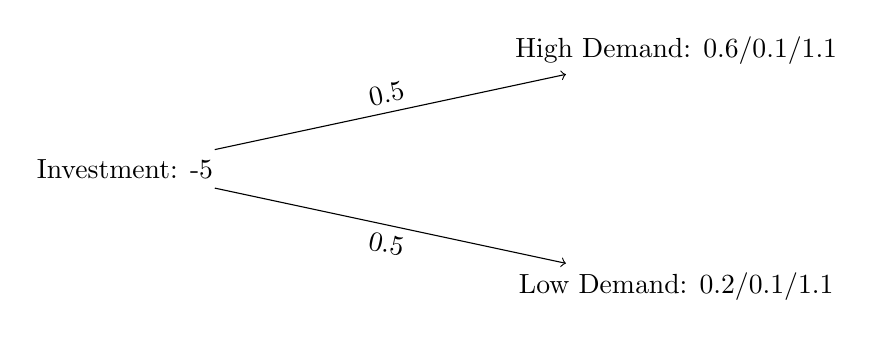
\begin{tikzpicture}[sloped]
        % Node definitions
        \node (a) at (0,0) {Investment: -5};
        \node (b) at (7,-1.5) {Low Demand: 0.2/0.1/1.1};
        \node (c) at (7,1.5) {High Demand: 0.6/0.1/1.1};

        % Edge definitions
        \draw [->] (a) to node [below] {0.5} (b);
        \draw [->] (a) to node [above] {0.5} (c);
    \end{tikzpicture}
    \caption{Option Tree for Investment Decision}
    \label{fig:option-tree}
    \end{figure}

    \textbf{Question: }
    What is the NPV? Should the CEO invest?\\
    \textbf{Answer: }
    \begin{align*}
        \text{NPV} &= -5 + 0.5 \times \left(\frac{0.6}{0.1 \times 1.1} \right) + 0.5 \times \left(\frac{0.2}{0.1 \times 1.1} \right) \\
        &= -1.36
    \end{align*}
    Negative NPV, so the CEO should not invest.\\

    \textbf{Question: }
    Now assume that the CEO has the option to delay the investment by one year to learn about demand levels, and can then decide whether or not to build the new plant. If she decides to wait one year to invest, the plant will only start to generate cash flows at the end of the third year. \\

    What is the new NPV and what is the value of the option to delay?

    \begin{figure}[H]
        \centering
        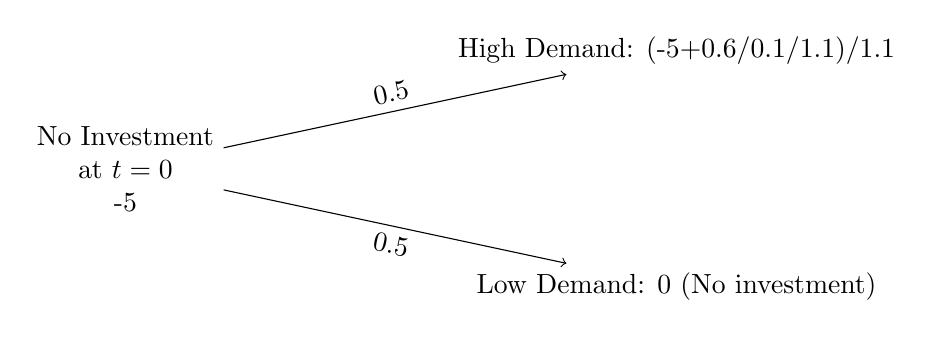
\begin{tikzpicture}[sloped]
            % Node definitions
            \node[align=center] (a) at (0,0) {No Investment \\ at $t=0$\\-5};
            \node (b) at (7,-1.5) {Low Demand: 0 (No investment)};
            \node (c) at (7,1.5) {High Demand: (-5+0.6/0.1/1.1)/1.1};
    
            % Edge definitions
            \draw [->] (a) to node [below] {0.5} (b);
            \draw [->] (a) to node [above] {0.5} (c);
        \end{tikzpicture}
        \caption{Option Tree for Investment Decision}
        \label{fig:option-tree-2}
    \end{figure}

    \textbf{Answer: }
    \begin{align*}
        \text{NPV} &= 0.5 \times \left(\frac{0.6}{0.1 \times 1.1} - 5\right) \\
        &= 0.207
    \end{align*}
    The value of the option to delay is $ 0.207 - (-1.36) = -1.57$.



\end{examplebox}
